\documentclass[12pt]{article}

\usepackage[utf8]{inputenc}
%\usepackage[T1]{fontenc}

\usepackage{geometry}
\geometry{a4paper}
\usepackage{graphicx}
\usepackage{float}
\usepackage[italian]{babel}

\linespread{1.2}
\setlength{\parindent}{0pt}

\begin{document}

\renewcommand{\labelenumii}{\arabic{enumi}.\arabic{enumii}}
\renewcommand{\labelenumiii}{\arabic{enumi}.\arabic{enumii}.\arabic{enumiii}}
\renewcommand{\labelenumiv}{\arabic{enumi}.\arabic{enumii}.\arabic{enumiii}.\arabic{enumiv}}
%----------------------------------------------------------------------------------------
%	TITOLO
%----------------------------------------------------------------------------------------

\begin{titlepage}

\newcommand{\HRule}{\rule{\linewidth}{0.5mm}}

\center

\textsc{\Large Relazione di progetto di "Smart City e Tecnologie Mobili"}\\[0.5cm]

\HRule \\[0.4cm]
{ \huge \bfseries CityTwin}\\[0.4cm]
\HRule \\[1.5cm]

\vfill

\begin{flushleft}
\emph{Numero del gruppo: 128}\\[1cm]
\emph{Componenti del gruppo: Eddie Barzi, Filippo Vissani}\\[3cm]
\end{flushleft}

\end{titlepage}

%----------------------------------------------------------------------------------------
%	INDICE
%----------------------------------------------------------------------------------------

\tableofcontents

\newpage

%----------------------------------------------------------------------------------------
%	INTRODUZIONE
%----------------------------------------------------------------------------------------

\section{Introduzione}

Il progetto CityTwin si propone di realizzare la simulazione di un sistema di digital twin nel contesto della smart city. In particolare, si vuole realizzare un sistema che sia in grado di catturare e rappresentare in formato digitale il comportamento delle varie entità presenti all'interno della città. Questo può portare ad una serie di benefici, alcuni dei quali vengono elencati di seguito:

\begin{itemize}
    \item Rilevazione di possibili problematiche e intervento tempestivo/automatizzato.
    \item Riduzione del consumo energetico.
    \item Rilevazione della qualità dell'aria e dell'acqua.
    \item Analisi dell'inquinamento acustico.
    \item Ottimizzazione della mobilità urbana.
\end{itemize}

La simulazione sarà composta da due tipologie di nodi: i nodi Mainstay, che rappresentano la struttura portante del sistema, e i nodi Resource, che rappresentano astrazioni di sensori, attuatori o entità più complesse.

I nodi Mainstay si occupano di scambiare informazioni con i nodi Resource, rilevare eventuali malfunzionamenti e salvare in modo persistente le informazioni rilevate dai nodi Resource. I nodi Mainstay devono essere sempre sincronizzati tra loro, in modo da poter garantire la coerenza dei dati.

I nodi Resource, invece, si occupano di rilevare informazioni e comunicarle ai nodi Mainstay nel caso in cui vengono considerati come sensori. Nel caso in cui i nodi Resource rappresentino attuatori, invece, si occupano di ricevere informazioni dai nodi Mainstay e agire di conseguenza.

Per la memorizzazione delle dello stato dei nodi viene disposto un servizio apposito di persistenza dei dati. Tale servizio viene utilizzato sia dai nodi Mainstay che da altri clienti, come ad esempio il pannello di controllo.

L'utente potrà visualizzare lo stato attuale del sistema, lo storico dei dati ed eventuali statistiche, nonché interagire con il sistema tramite GUI, ad esempio per intervenire dopo la rilevazione di un incendio.

Per la realizzazione del progetto verranno utilizzate le seguenti tecnologie:

Akka è un toolkit open source e runtime che semplifica la costruzione di applicazioni concorrenti e distribuite sulla JVM. Questo toolkit supporta diversi modelli di programmazione per la concorrenza, ma enfatizza la concorrenza basata su attori.

I componenti principali del progetto, quali Mainstay e Resource, verranno modellati sulla base del paradigma ad attori e verranno realizzati utilizzando Akka in combinazione con il linguaggio Scala 3.

Per quanto riguarda il servizio di persistenza dei dati, utile per visualizzare le statistiche, verrà utilizzato MongoDB, un database non relazionale orientato ai documenti. Questo database verrà utilizzato per salvare in modo persistente i dati rilevati dai nodi Mainstay.
Il servizio di persistenza verrà realizzato come modulo separato, per questo motivo si sceglie di implementare un layer scritto in JavaScript, che esponga delle API utilizzabili sia dai nodi Mainstay che da altri clienti.

Sulla base dei linguaggi scelti, verranno adottati Simple Build Tool (SBT) per Scala 3 e Node Package Manager (NPM) per JavaScript per la gestione delle dipendenze e la compilazione del codice.

Per semplificare l'avvio del sistema distribuito e garantire la scalabilità verrà utilizzato Docker, un progetto open source che automatizza il deployment di applicazioni all'interno di contenitori software.

\newpage

%----------------------------------------------------------------------------------------
%	STATO DELL'ARTE
%----------------------------------------------------------------------------------------

\section{Stato dell'arte}

Riassumere le soluzioni presenti in letteratura inerenti al problema in esame. Per ciascuna, discutere le principali diversità o affinità rispetto al progetto presentato. Nel caso non siano presenti soluzioni direttamente comparabili a quella presentata descrivere comunque le principali tecniche note per affrontare la tematica trattata.\\

Le soluzioni esposte devono essere corredate degli opportuni riferimenti bibliografici. Nel caso si tratti di soluzioni già operative sul mercato, devono essere indicate le fonti (online) dove poter accedere al servizio o approfondirne i contenuti.\\


Vincoli circa la lunghezza della sezione (escluse didascalie, tabelle, testo nelle immagini, schemi):

\vspace{1cm}
\begin{tabular}{l|rr}
 & Numero minimo di battute & Numero massimo di battute \\
 \hline
 1 componente & 2000 & 3000 \\
 2 componenti & 2500 & 4500 \\
 3 componenti & 3000 & 6000 \\
 \hline
\end{tabular}


\newpage


%----------------------------------------------------------------------------------------
%	ANALISI DEI REQUISITI
%----------------------------------------------------------------------------------------

\section{Analisi dei requisiti}

Di seguito viene riportato l'elenco dettagliato dei requisiti del sistema.

\begin{enumerate}
    \item I nodi Mainstay sono la struttura portante dell'intero sistema:
    \begin{enumerate}
        \item Ricevono informazioni dai nodi Resource che modellano sensori.
        \item Comunicano informazioni ai nodi Resource che modellano attuatori.
        \item Rilevano i malfunzionamenti dei nodi Resource.
        \item Rilevano i malfunzionamenti degli altri nodi Mainstay.
        \item Si occupano di salvare le informazioni contattando il servizio di persistenza.
        \item Non devono conoscere a prescindere le tipologie dei nodi Resource.
        \item Devono disporre di una struttura dati distribuita che permetta di memorizzare le informazioni rilevanti:
        \begin{enumerate}
            \item La struttura dati deve essere sincronizzata tra i nodi Mainstay.
            \item La struttura dati deve mantenere la consistenza dei dati nel tempo.
        \end{enumerate}
    \end{enumerate}
    \item I nodi Resource:
    \begin{enumerate}
        \item Rappresentano astrazioni di:
        \begin{enumerate}
            \item Sensori.
            \item Attuatori.
            \item Entità più complesse, come stazioni di controllo, che possono anche impiegare interfacce grafiche.
        \end{enumerate}
        \item Fanno riferimento ad uno dei nodi Mainstay per ottenere o comunicare informazioni.
        \item Possono essere aggiunti o rimossi in tempo reale.
    \end{enumerate}
    \item Deve essere presente una GUI (distinta da quelle definite al punto 2.1.3) con le seguenti funzionalità:
    \begin{enumerate}
        \item Deve mostrare lo stato attuale dei nodi Mainstay e Resource del sistema.
        \item Deve mostrare la posizione delle risorse nella città.
        \item Deve presentare alcune statistiche interessanti sulla base dei dati rilevati dal servizio di persistenza.
    \end{enumerate}
    \item Deve essere presente un servizio di persistenza dei dati che permetta di salvare in modo persistente:
    \begin{enumerate}
        \item Lo stato dei nodi Mainstay.
        \item Lo stato dei nodi Resource.
    \end{enumerate}
    \item Il malfunzionamento di un nodo non deve compromettere il funzionamento del sistema.
    \item Il sistema deve essere realizzato in moduli separati, in modo da poter essere facilmente estendibile.
    \item Deve poter essere possibile introdurre nuovi moduli senza dover modificare i componenti esistenti.
    \item Vengono previsti i seguenti moduli per i nodi Resource:
    \begin{enumerate}
        \item Sensore per la rilevazione di piogge acide.
        \item Sensore per l'analisi della qualità dell'aria.
        \item Sensore per la rilevazione dell'inquinamento acustico.
        \item Modulo per la rilevazione del livello dell'acqua di un fiume e possibilità di intervento:
        \begin{enumerate}
            \item Sensore per la rilevazione degli allagamenti.
            \item Pannello di controllo per l'intervento in caso di allagamento.
        \end{enumerate}
    \end{enumerate}
\end{enumerate}

\newpage


%----------------------------------------------------------------------------------------
%	PROGETTAZIONE
%----------------------------------------------------------------------------------------

\section{Progettazione}

\begin{figure}[t]
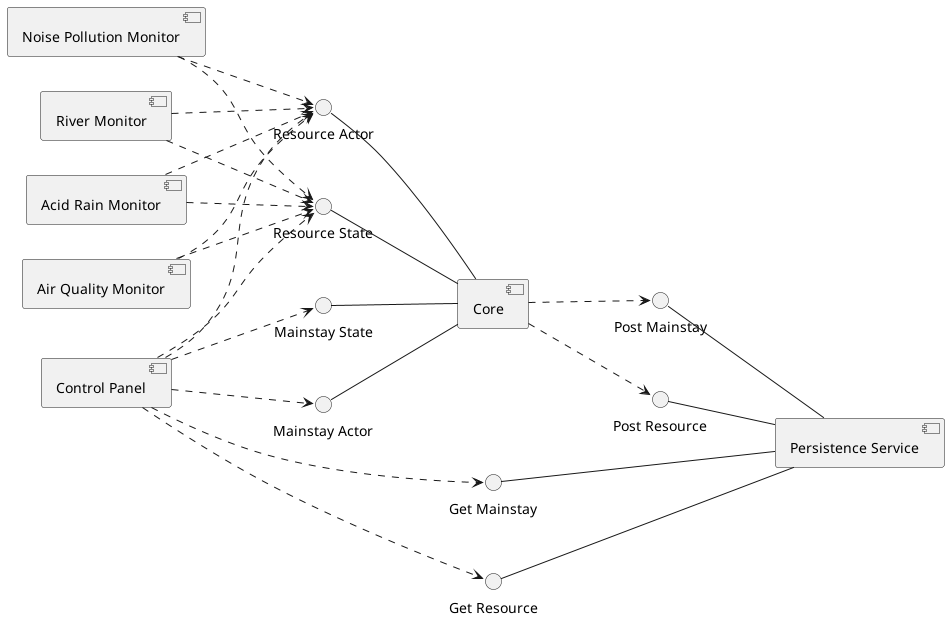
\includegraphics[width=\textwidth]{../assets/images/core-component-diagram.png}
\end{figure}

\begin{figure}[t]
    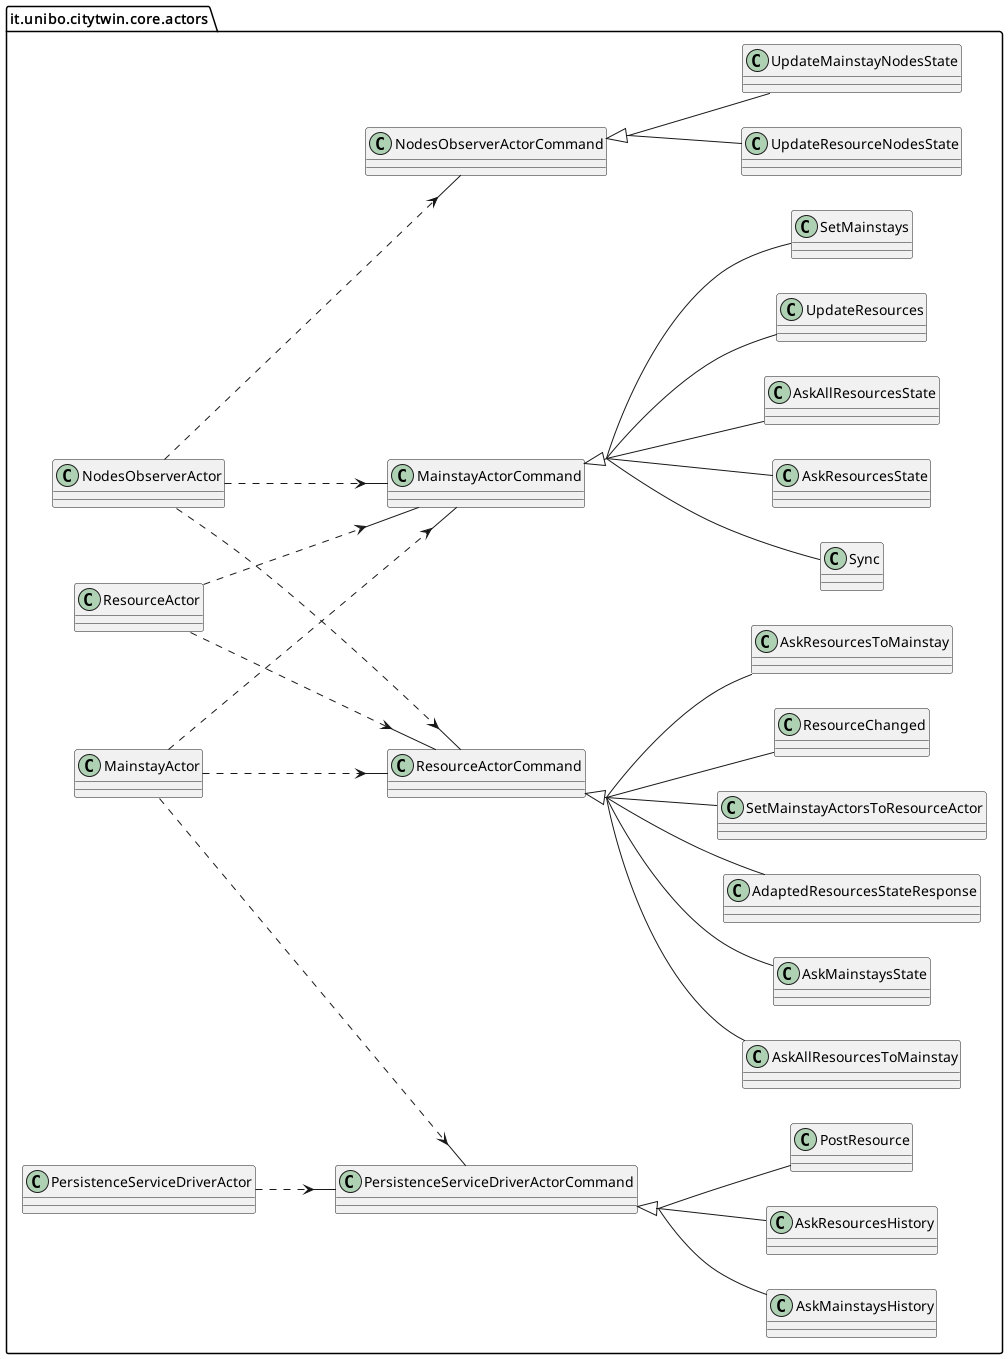
\includegraphics[width=\textwidth]{../assets/images/core-class-diagram.png}
\end{figure}

\begin{figure}[t]
    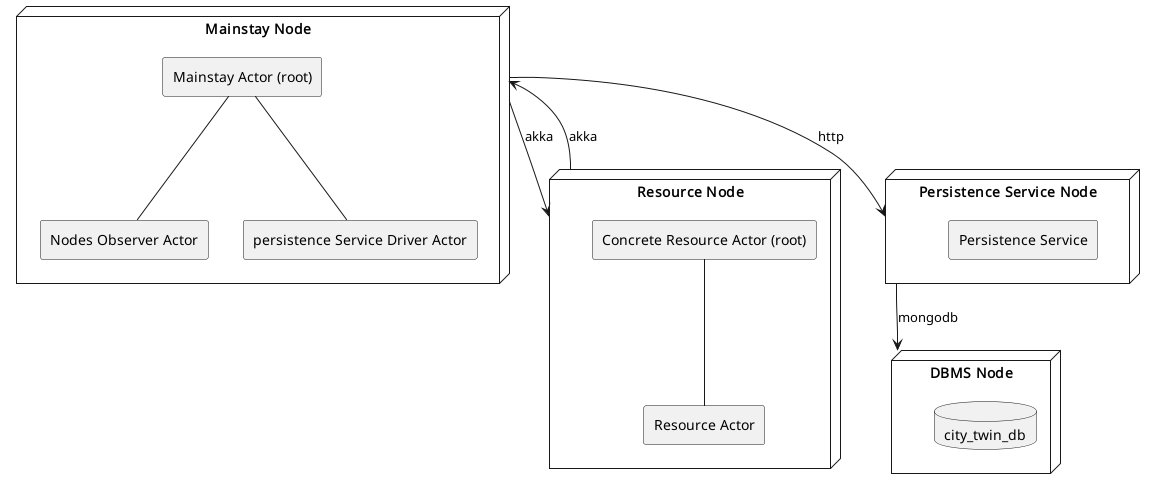
\includegraphics[width=\textwidth]{../assets/images/nodes-component-diagram.png}
\end{figure}

\begin{figure}[t]
    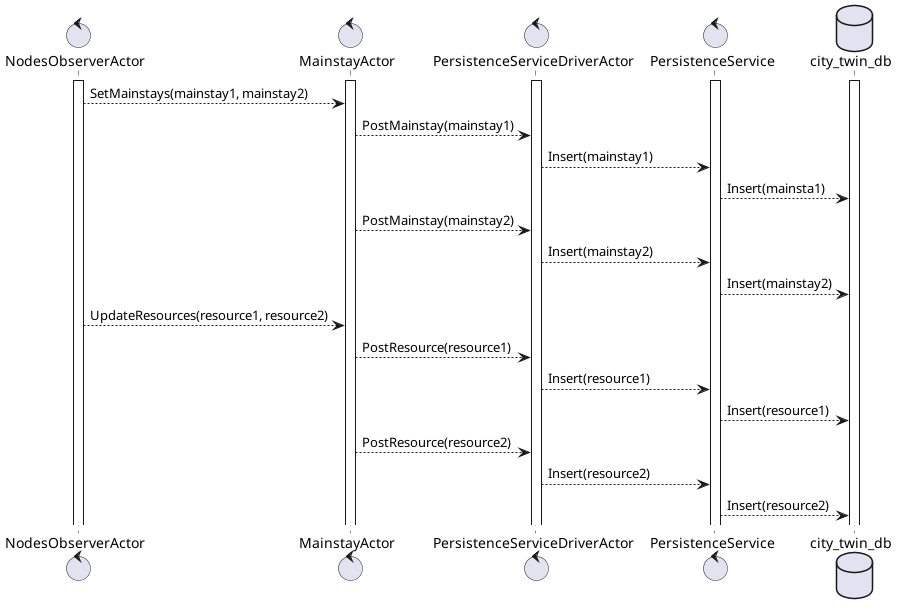
\includegraphics[width=\textwidth]{../assets/images/core-nodes-state-sequence-diagram.png}
\end{figure}

\begin{figure}[t]
    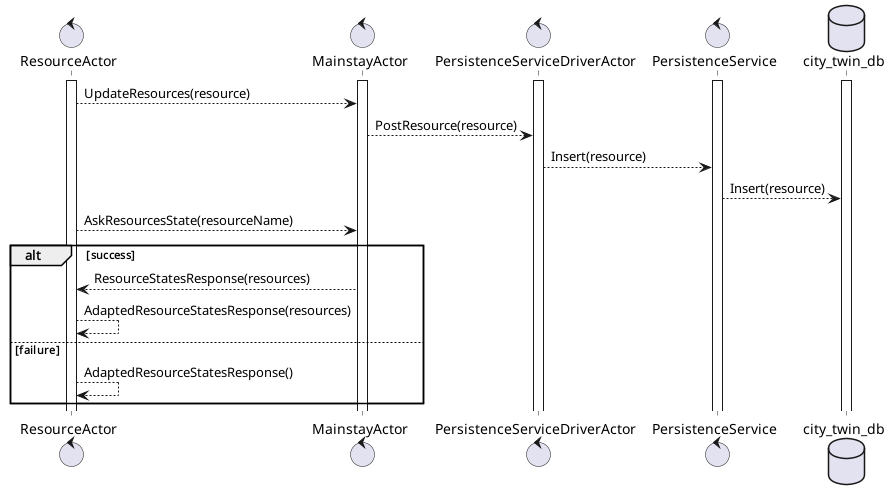
\includegraphics[width=\textwidth]{../assets/images/core-resource-state-exchange-sequence-diagram copy.png}
\end{figure}

\begin{figure}[t]
    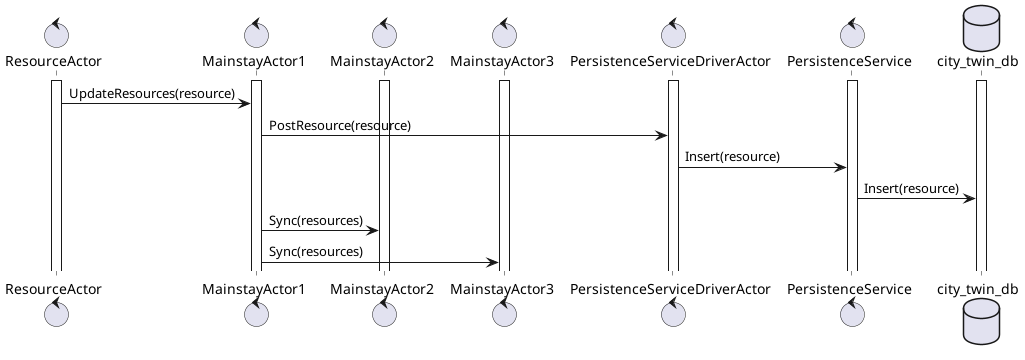
\includegraphics[width=\textwidth]{../assets/images/core-mainstays-sync-sequence-diagram.png}
\end{figure}

\newpage

%----------------------------------------------------------------------------------------
%	IMPLEMENTAZIONE
%----------------------------------------------------------------------------------------

\section{Implementazione}\label{sec:implementazione}

Esporre i principali problemi affrontati durante l'effettiva realizzazione delle componenti hardware/software e illustrare le soluzioni implementative adottate. Se l'elaborato ha previsto l'utilizzo di tecnologie già disponibili sul mercato, discuterne brevemente le caratteristiche e motivarne l'adozione rispetto ad altre soluzioni assimilabili.\\

\textbf{NOTA: in questa sezione devono essere riportate esclusivamente le porzioni di codice ritenute particolarmente significative. Il codice sorgente nella sua interezza, opportunamente commentato, deve essere consegnato separatamente dalla relazione in un archivio compresso.}\\


Vincoli circa la lunghezza della sezione (escluse didascalie, tabelle, testo nelle immagini, schemi):

\vspace{1cm}
\begin{tabular}{l|rr}
 & Numero minimo di battute & Numero massimo di battute \\
 \hline
 1 componente & 5000 & 11000 \\
 2 componenti & 8000 & 16000 \\
 3 componenti & 10000 & 21000 \\
 \hline
\end{tabular}


\newpage


%----------------------------------------------------------------------------------------
%	TESTING E PERFORMANCE
%----------------------------------------------------------------------------------------

\section{Testing e performance}

Esporre lo stato di funzionamento effettivo del sistema progettato ad elaborato concluso. Per ciascuna delle funzionalità salienti devono essere tabellate e discusse le performance riscontrate mediante opportuni test eseguiti in fase di validazione del progetto.\\

I tempi di esecuzione/comunicazione devono essere accompagnati dalle caratteristiche dell'hardware sul quale è eseguito il software.\\

Qualora l'elaborato includa algoritmi innovativi, indicarne la complessità computazionale (avendo cura di esporre lo pseudo codice nella sezione \ref{sec:implementazione}).\\


Vincoli circa la lunghezza della sezione (escluse didascalie, tabelle, testo nelle immagini, schemi):

\vspace{1cm}
\begin{tabular}{l|rr}
 & Numero minimo di battute & Numero massimo di battute \\
 \hline
 1 componente & 2000 & 3000 \\
 2 componenti & 2500 & 4500 \\
 3 componenti & 3000 & 6000 \\
 \hline
\end{tabular}


\newpage


%----------------------------------------------------------------------------------------
%	ANALISI DI DEPLOYMENT SU LARGA SCALA
%----------------------------------------------------------------------------------------

\section{Analisi di deployment su larga scala}

In questa sezione va discussa, eventualmente con l'ausilio di opportuni diagrammi (componenti, deployment), l'evoluzione del progetto presentato immaginando che venga adottato su larga scala. I dettagli qui esposti devono quindi astrarre dalle specifiche dell'elaborato qualora l'implementazione sia stata focalizzata su uno scenario isolato.\\

A titolo d’esempio, qualora applicabile, devono essere evidenziate le criticità che si potrebbero incontrare e devono essere proposte soluzioni tipiche in contesti di \textit{cloud architecture} per garantire un'adeguata \textit{resilienza}, in termini di \textit{availability} e \textit{scalability} del sistema.\\


Vincoli circa la lunghezza della sezione (escluse didascalie, tabelle, testo nelle immagini, schemi):

\vspace{1cm}
\begin{tabular}{l|rr}
 & Numero minimo di battute & Numero massimo di battute \\
 \hline
 1 componente & 3000 & 6000 \\
 2 componenti & 4500 & 9000 \\
 3 componenti & 6000 & 12000 \\
 \hline
\end{tabular}


\newpage


%----------------------------------------------------------------------------------------
%	PIANO DI LAVORO
%----------------------------------------------------------------------------------------

\section{Piano di lavoro}

In questa sezione devono essere chiariti i compiti svolti da ciascun candidato nel caso in cui il gruppo abbia più di un componente.\\

Deve essere inoltre esposto il piano di lavoro adottato. A tal fine, per ogni attività svolta durante la preparazione dell'elaborato (ad esempio: studio di una tecnologia, progettazione di un componente, implementazione di un algoritmo ecc…) deve essere chiarita la collocazione temporale e devono essere indicate le risorse impiegate per svolgerla (giorni/uomo). I candidati possono ricorrere a opportuni diagrammi come quello di Gantt.\\


Vincoli circa la lunghezza della sezione (escluse didascalie, tabelle, testo nelle immagini, schemi):

\vspace{1cm}
\begin{tabular}{l|rr}
 & Numero minimo di battute & Numero massimo di battute \\
 \hline
 1 componente & 1000 & 2000 \\
 2 componenti & 1500 & 3000 \\
 3 componenti & 2000 & 4000 \\
 \hline
\end{tabular}

\newpage


%----------------------------------------------------------------------------------------
%	CONCLUSIONI
%----------------------------------------------------------------------------------------

\section{Conclusioni}

Esporre brevemente le considerazioni conclusive sul progetto presentato, indicando anche i possibili sviluppi futuri.\\

Vincoli circa la lunghezza della sezione (escluse didascalie, tabelle, testo nelle immagini, schemi):

\vspace{1cm}
\begin{tabular}{l|rr}
 & Numero minimo di battute & Numero massimo di battute \\
 \hline
 1 componente & 500 & 1000 \\
 2 componenti & 1000 & 2000 \\
 3 componenti & 1500 & 3000 \\
 \hline
\end{tabular}

\newpage


%----------------------------------------------------------------------------------------
%	APPENDICE
%----------------------------------------------------------------------------------------

\appendix
\addcontentsline{toc}{section}{Appendice}
\section*{Appendice}
Laddove necessario è possibile avvalersi di appendici alla relazione per includere materiale di approfondimento.\\

A titolo esemplificativo possono essere incluse le schede tecniche dei componenti adottati, la normativa di riferimento che regola un particolare dominio applicativo, ecc.


\newpage


%----------------------------------------------------------------------------------------
%	RIFERIMENTI BIBLIOGRAFICI
%----------------------------------------------------------------------------------------
\addcontentsline{toc}{section}{Riferimenti bibliografici}
\begin{thebibliography}
EElencare i riferimenti bibliografici citati nel testo. 
\end{thebibliography}

%----------------------------------------------------------------------------------------

\end{document}